\chapter{The CLI-Tutor Tool}
% - Tool (CLI-Tutor)
%   - overview
%       - curriculum
%       - lesson design
%            - deliberate emphasis on  easy vocabulary
%            - running examples
%            - refresher from previous lesson
%       - usability considerations
%       - safety considerations
%       - vocab and validation
%   - web version
%
\label{chap:clitutor}

\begin{lstlisting}[float=htbp, keepspaces, frame=single, language={}, label=lst:clihelp, caption=Output of the help flag of \textit{CLI-Tutor} running in a docker container.]
cli-student@3bc86f9090f9:~/tutor$ cli-tutor -h

        _ _       __        __
  _____/ (_)     / /___  __/ /_____  _____
 / ___/ / /_____/ __/ / / / __/ __ \/ ___/
/ /__/ / /_____/ /_/ /_/ / /_/ /_/ / /
\___/_/_/      \__/\__,_/\__/\____/_/

A simple command line tutor application that aims to introduce users to the
    basics of command line interaction.
    Web version is available at https://clitutor.chistole.ch

Usage:
  cli-tutor [flags]
  cli-tutor [command]

Available Commands:
  completion  Generate the autocompletion script for the specified shell
  help        Help about any command
  info        Prints information about the tool and log collection
  repo        Prints a url to the git repository for this tool
  version     Print the version number of cli-tutor

Flags:
  -h, --help            help for cli-tutor
  -n, --no-upload-log   Do not send a copy of the log to the developer
  -x, --no-welcome      Do not show welcome message when entering tutor

Use "cli-tutor [command] --help" for more information about a command.
\end{lstlisting}

\textit{CLI-Tutor} is a command line application written in the \textit{Go}
programming language. It is an interactive tutorial focused on introducing
novices to the Linux command line environment. The application is intended to
be a forgiving but faithful representation of a shell running
\textit{Bash}\footnote{\textit{Bourne Again SHell}:
\url{https://www.gnu.org/software/bash/}}. In this chapter, we will discuss the
semantic design considerations and choices made during the development of
\textit{CLI-Tutor}.

\section{Overview}
\subsection{Curriculum}

%feedback here was to summarize lessons in one sentence, is this still necessary.
\textit{CLI-Tutor} is intended to be used with zero prerequisite knowledge of
the command line. To achieve this low barrier to entry, lessons are designed
from the perspective of catering to a complete novice user. The curriculum
consists of lessons that introduce the very basics of textual interaction and
shell usage. As of writing, \textit{CLI-Tutor} has 5 full lessons implemented
as a proof of concept and serve as the curriculum in the user study conducted
in this thesis work. \textit{CLI-Tutor} is designed to be easily extensible
with new lessons being easy to contribute. How this is achieved will be
discussed later in \autoref{chap:design}.

\subsubsection{Summary of implemented lessons}

\paragraph{Basics of Textual Interaction.} This lesson covers the very
foundational concepts of textual interaction. The user is introduced to the
term \textit{CLI} and explained what a \textit{shell} is using an ASCII
graphic. The user is then introduced to the concept of issuing a command. To
sow interest, the user is then asked to execute some commands to illustrate that
the terminal is really interacting with their operating system. The Users are
asked to use the \textit{curl} from command to pull down a weather report from
the \url{wttr.in} as an example of what is possible with the command line.
Furthermore, the user is introduced to some important in-built commands
of \textit{CLI-Tutor} and taught how to clear the screen. Another feature
introduced to the user is \textit{zen-mode}, a feature that prevents the screen
from being cluttered with output of previous commands to prevent the user from
getting overwhelmed. This feature is activated by default in lesson 1 but is
then deactivated, unless explicitly set, for the remainder of the curriculum.

\paragraph{Getting more familiar with the shell.} This lesson jumps deeper into
the concept of issuing commands and the "grammar" behind a command. To make
this more intuitive the metaphor of a sentence is used, adapted from the
documentation of the \textit{cobra} command line tool
library\cite{franciacobra}. The lesson introduces users to fundamental concepts
such as sub-commands and flags. The user is then asked to perform a series of
tasks involving the \textit{wc} word counting core utility. These actions are
performed on a sample file that \textit{CLI-Tutor} creates and serves as a
running example throughout the tutor.

\paragraph{Basics of the file system and practising commands.} Lesson 3 is all
about the file system and file system operations. The user is first introduced
to the prompt and explained all the different sections of the prompt line. The
prompt in \textit{CLI-Tutor} is modelled after the stock prompt of many popular
Linux distributions (see: \autoref{lst:clihelp}, line 1), consisting of a
username, hostname and current working directory path. The user is introduced
to the idea of a hierarchical tree-like file system and is taught how to
navigate around it. The \textit{ls} command is also discussed and used to
illustrate the concept of hidden files. \textit{CLI-Tutor} also includes a
hidden file that it places in the directory the tutor is launched from to help
illustrate the concept of hidden files. All the example files included in
lessons are deleted upon exiting the tutor. The lesson closes with a long
example for the user to try out that includes all the concepts discussed in the
lesson.

\paragraph{Shell shortcuts and tricks.} This lesson is aimed to be a bit more
fun and introduces the user to some tricks and shortcuts available in the shell
and the \textit{readline}\cite{ramey_fox_readline} library used for input in a
\textit{bash} shell environment. The user is introduced to the concept of a
shell history file and also of the reverse history search feature with
\textit{Ctrl+r}. The cancel \textit{Ctrl+c} command is introduced as well
as the \textit{!!} operator. As a final step, tab completion is introduced.

\paragraph{Helping yourself.} This is the last lesson of the current version of
\textit{CLI-Tutor} and covers how a user can go about seeking help at the
command line and helping themselves. The concept of pagers and some important
keybindings of the \textit{less} pager program are first explained before
introducing the \textit{man} command to the user. Users are also taught about
help flags and encouraged to check out the help command of \textit{CLI-Tutor},
shown at the very beginning of this \hyperref[chap:clitutor]{chapter} (see:
\autoref{lst:clihelp}).

%TODO: Maybe move or delete first two lines
\subsection{Lesson Design} Lessons in \textit{CLI-Tutor} are written as a
Markdown files and are rendered in the lesson view by a Markdown renderer. The
exact structure of this Markdown file will be discussed in
\autoref{chap:design} (see: \autoref{lst:markdown}). Lessons are designed to
cover one topic per lesson and  consist of a bit of introduction to the concept
before jumping into directly applying the subject in a series of interactive
tasks. Each lesson, typically, also starts with a very short refresher of the
last lesson and ends with a recap of the learnt commands. The lessons are
designed to be guided but to leave some room for exploration for the user.
\textit{CLI-Tutor} also has some running examples that are included in the form
of files that are created upon launching the program and deleted when the
program exits. These files are included in for the purpose of augmenting the
tasks and to allow the user to directly apply commands rather than creating an
environment to support their learning themselves.

\subsubsection{Anatomy of a lesson} A lesson consists of a series of tasks.
Some of these tasks are purely educational and aim to teach the concept being
covered in the lesson and some tasks are interactive. Generally, each
task tries to build upon the previous. While writing the lessons, there was a
deliberate emphasis on keeping the text short and engaging. The goal was to
focus on the interactivity and not to provide long text passages for the user
to read. In order to achieve this succinctness, the use of examples, metaphors
and formatted text to convey ideas was crucial.

\subsubsection{Lessons also contain two additional features:}

\paragraph{Vocabulary.}  The vocabulary of a lesson is the set of permitted
commands in that lesson. This is primarily designed as a safety feature to
prevent users from issuing commands incorrectly or bringing damage to their
systems. The vocabulary consists of commands that will be covered in the
current lesson and also commands previously covered in the tutor.

\paragraph{Expected values.} Expected values are what drive the interactivity
of \textit{CLI-Tutor}. Expected values prompt the tutor to consider the current
task as interactive and thus the tutor blocks advancing to the next task unless
the interactive task is performed. The expected value pertains to the expected
result of performing a certain command or action. This expected value can be
specified in three different ways (see: \autoref{lst:markdown}). Expected values could be a constant values such
as a string or number, they could be the result of some function call and even
a system call.

\subsection{Usability Considerations}

As previously mentioned, lessons are designed with no prior knowledge
assumption. In addition to the curriculum a number of considerations regarding
the usability and design of the tool also had to be taken to maintain a very
low barrier to entry.

\subsubsection{User Interface} In general, the user interface of
\textit{CLI-Tutor} is designed to be very simple and uncluttered. Strictly
speaking, despite aiming to be an application that mimics a shell environment,
\textit{CLI-Tutor} is a \textit{TUI} or "Text User Interface" application. A
TUI application is a command line application that typically takes control of
the entire terminal window and may contain some graphical elements. In the case
of \textit{CLI-Tutor}, the menu view contains a graphical list that is
"hoverable" and clickable. The lesson view also takes control of the entire
terminal window to render text to the screen.  It consists of two primary
views, the lesson view and the menu view. Special consideration had to be given
to the user interface to make it not only new user-friendly, but also a fair
representation of a terminal environment. Unlike tutorial software designed for
programming languages, which tend to not have their own distinct environment,
the shell is very much its own environment. Helping a user become familiar with
the shell environment is important if the intimidation factors are to be
overcome.

\paragraph{Menu view.} The menu view is what the user is greeted with upon
launching the program. It lists the lessons in a menu which the user can use to
select and start a lesson (see: \autoref{fig:clitutormenu}). The menu view also
has a help bar at the base with the keyboard shortcuts illustrated and allows
for filtering the lessons by using the search functionality. Menu items display
the title and description of a lesson, which are parsed directly from the
Markdown-based lesson files.

\begin{figure}[htbp]
	% \begin{figure}[H]
	\centering
	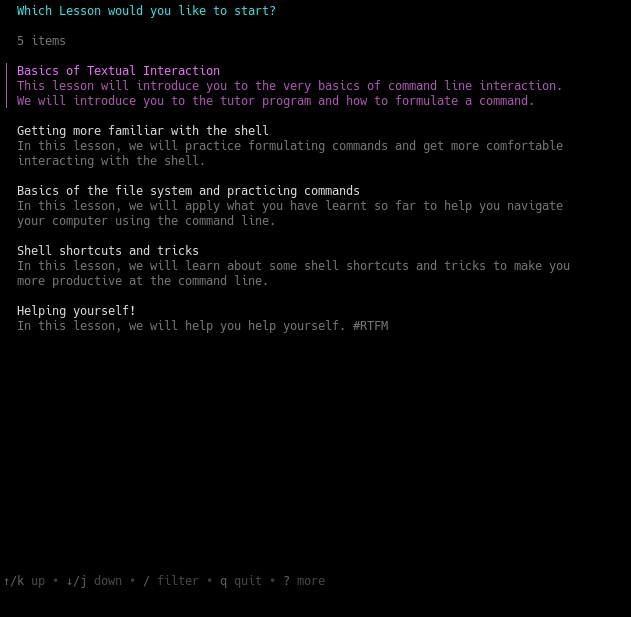
\includegraphics[width=0.9\textwidth]{img/menushort}
	\caption{Screenshot of \textit{CLI-Tutor} menu screen.}
	\label{fig:clitutormenu}
\end{figure}


\paragraph{Lesson view.} The lesson view is where the shell environment is
reproduced. It is designed to look exactly like what interacting with the shell
in a terminal looks like but with some added cues from the lesson. These cues
include the current task, its instructions and any feedback about the last
input of the user (see: \autoref{fig:lessonview}). The lesson view is also
running a \textit{Go} \textit{readline} library to provide a user input
mechanism essentially identical to that of a normal shell. The expected
shortcuts all work as they should but certain controls such as \textit{Ctrl+d},
\textit{Ctrl+z} and the \textit{Ctrl+c} interrupts are captured and ignored in
order to not close the program unexpectedly.

\begin{figure}[htbp]
	% \begin{figure}[H]
	\centering
	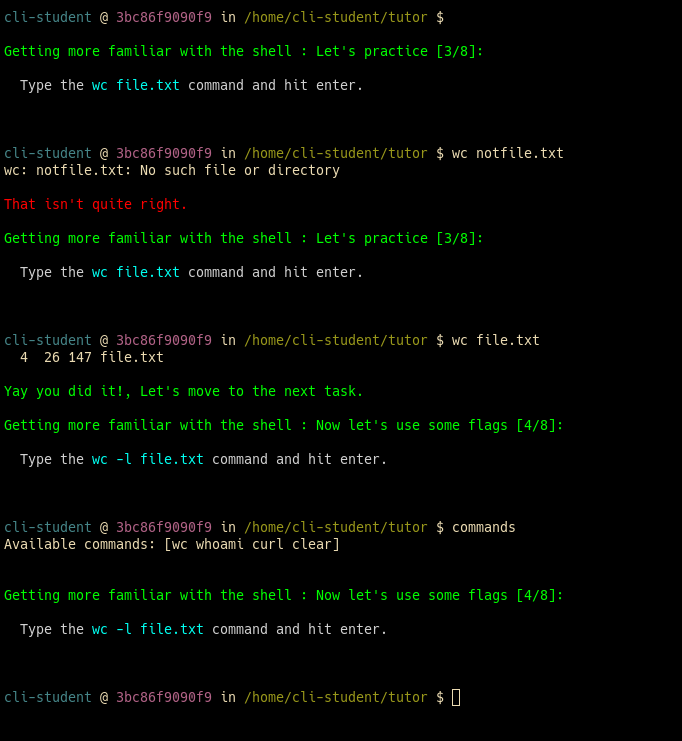
\includegraphics[width=0.9\textwidth]{img/lessonview}
	\caption{Screenshot of the \textit{CLI-Tutor} lesson view showing the task tracker, feedback mechanism and an inbuilt helper command.}
	\label{fig:lessonview}
\end{figure}


\paragraph{Mouse support.} To make the program more usable for
individuals used to GUIs, basic mouse support had to be implemented in
\textit{CLI-Tutor}. Mouse support is a bit extended in the menu than what would
be common in most TUI applications. The user can hover to highlight and click
to select a lesson. The hitboxes for the menu items are also precisely
calculated based on the text rendered to offer a consistent and GUI-like mouse
experience. In the lesson view, mouse support is implemented to a degree but
still retains the goal of providing an honest shell-like experience. The user
can access the scrollback buffer and use the mouse to select and copy text
using the keyboard shortcuts of their terminal emulator. In the web version, a
right-click menu that is native to the browser is also available.

\paragraph{Keyboard shortcuts (multiple for same).} As shown in
\autoref{fig:lessonview}, some inbuilt commands available to the user, are
not shell commands. For example, the \textit{commands} command prints all the
available commands, also known as the lesson's \textit{vocabulary}, to the
screen. There are other special commands in the lesson view that allow the user
to navigate forward and backwards through the lesson, quit the lesson and
toggle \textit{zen-mode}.

\paragraph{Zen mode.} This is a special output printing mode of the lesson
view. While not something available by default in a shell, this feature aims to
prevent the user from being overwhelmed by long textual output alongside the
lesson instructions. When \textit{zen-mode} is activated, the screen clears
itself before the output of every command. This has the effect of leaving only
the latest output and task on the screen. This feature is activated by default
in the very first lesson but then deactivated unless specifically set once the
user has been taught about clearing the screen using the \textit{clear}
command.

\paragraph{Feedback colouring.} \textit{CLI-Tutor} utilises colour to
differentiate different elements of the lesson. For example, a cyan colour is
used to indicate commands, green is used for the task tracker, yellow is used
for notes or information about key bindings and finally success and failure
feedback is also coded in red and green respectively (see:
\autoref{fig:lessonview} and \autoref{fig:colours}). In addition to colour,
text formatting elements such as the use of bold and italic text is also
utilised to form visual hierarchies and to attract the user's attention.


\subsection{Safety Considerations}

\paragraph{Fake jail warden.} To minimise the disruptions caused by
file permissions issues that may be completely cryptic to the user
\textit{CLI-Tutor}  uses a fake jail to prevent the current working directory
from being moved above the home folder of the user.

\paragraph{Sandbox.} In addition to permissions issues which are merely an
inconvenience, accidental file deletion or other potential mistakes during a
file system lesson can result in permanent data loss. To mitigate this risk and
to create a safe "sandbox" for users to use the application. The simplest
way is to run the application in a \textit{docker}\cite{dockerinc_2022}
container. However, this greatly increases the barrier of entry to using
\textit{CLI-Tutor}. To make the tool accessible and easy to distribute
a web application to serve instances of \textit{docker} containers running
\textit{CLI-Tutor} was created.

\section{Web Application}

While the core component of \textit{CLI-Tutor} is a command line application it
does have an accompanying web application (see: \autoref{fig:webversion}). The
purpose of creating this web application was briefly discussed in the preceding
section. The web application was the medium through which the user study was
conducted. Two versions of the web application were created to support the two
user groups in the user study (see: \autoref{chap:userstudy}). One version
contains the \textit{CLI-Tutor} program and the second "CLI only" version (see: \autoref{fig:cliversion})
serves to provide a sandboxed Linux shell to individuals participating in the
user study. Additionally, also to support the User Study a documentation static
website (see: \autoref{fig:docsweb}) was also created alongside the web application. In this section, we
will describe the general architecture of the application. More technical
details will be discussed in \autoref{chap:design}.


\begin{figure}[htbp]
	\centering
	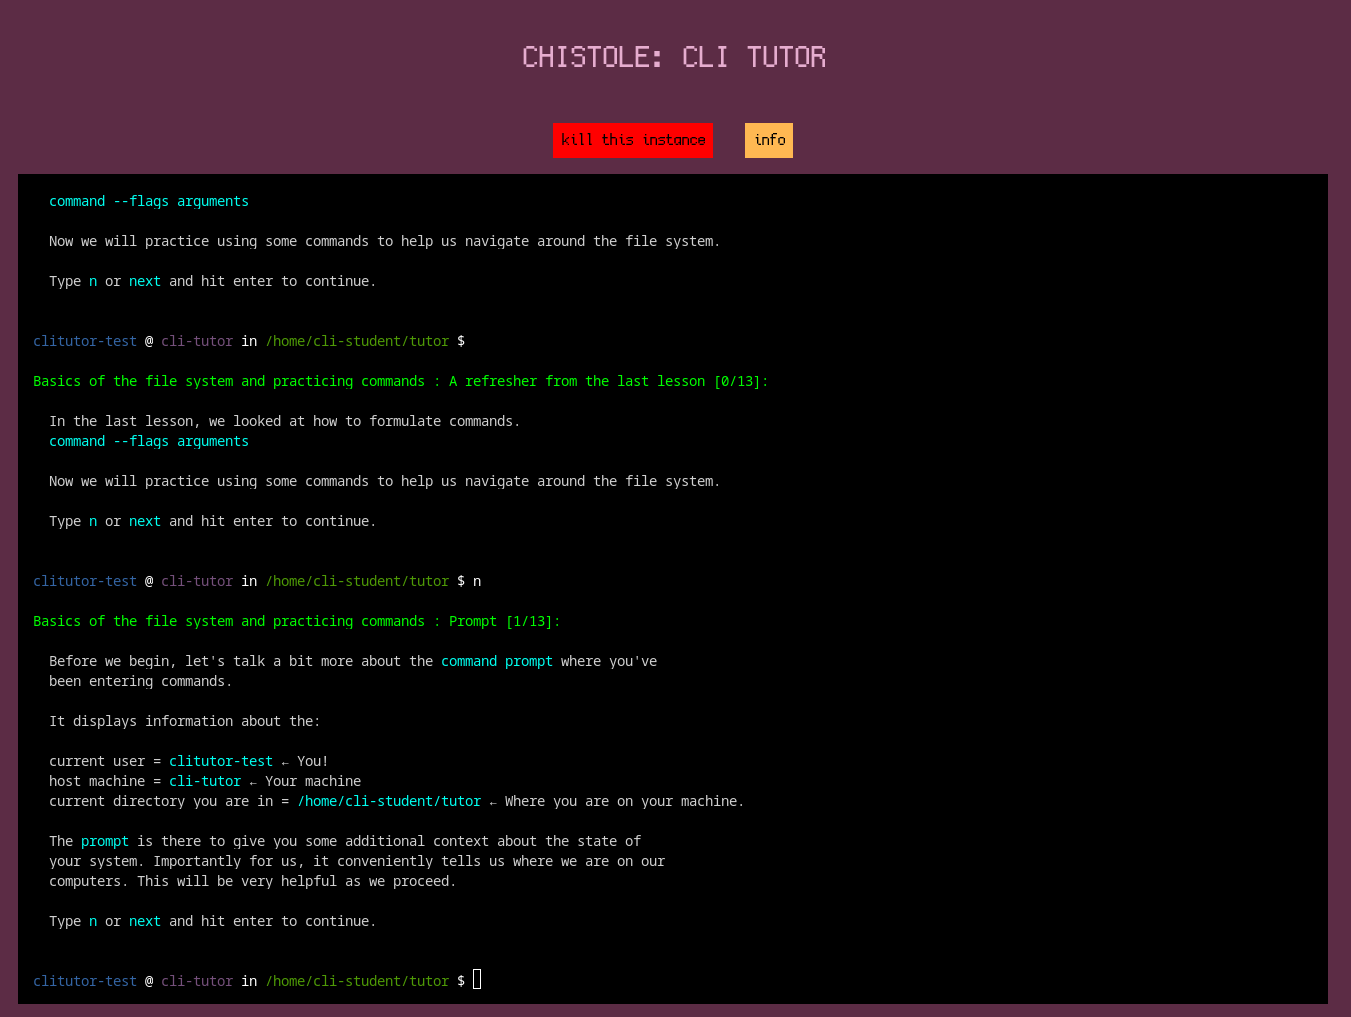
\includegraphics[width=1\textwidth]{img/cliwebshort}
	\caption{Screenshot of \textit{CLI-Tutor} running in a browser.}
	\label{fig:webversion}
\end{figure}

\begin{figure}[htbp]
	\centering
	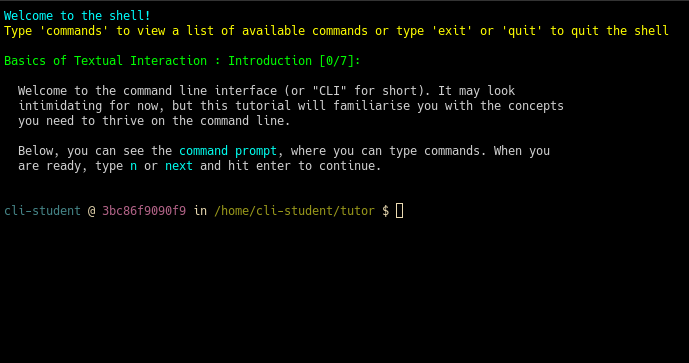
\includegraphics[width=0.9\textwidth]{img/lesson1.1}
	\caption{Screenshot of \textit{CLI-Tutor} showcasing the usage of colours.}
	\label{fig:colours}
\end{figure}

\begin{figure}[htbp]
	\centering
	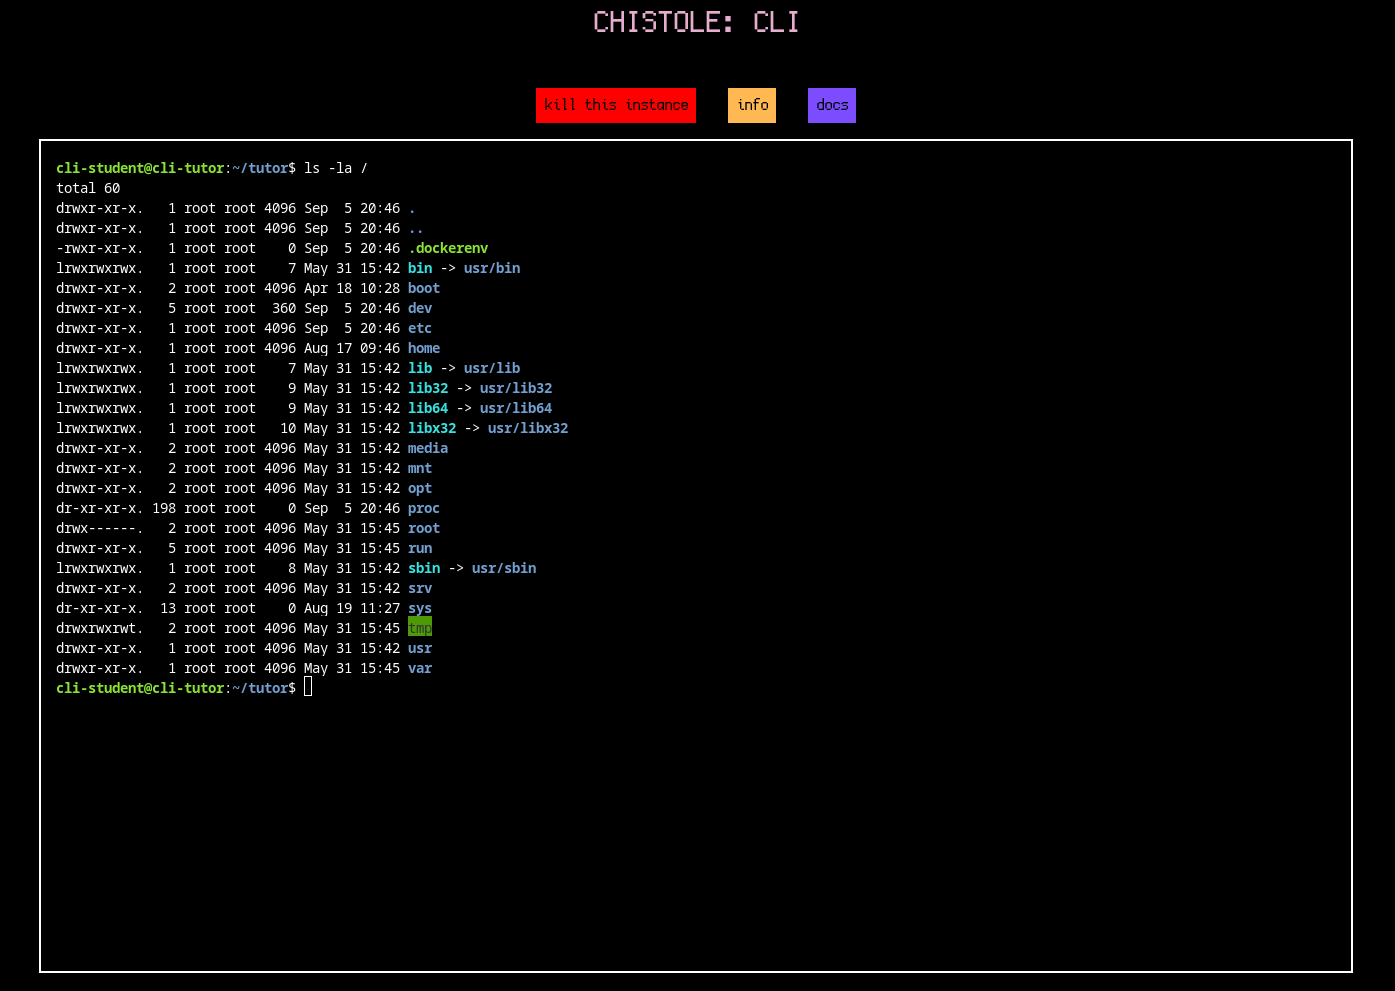
\includegraphics[width=1\textwidth]{img/clionly}
	\caption{Screenshot of the CLI only version.}
	\label{fig:welcomedocs}
\end{figure}
\begin{figure}[htbp]
	\centering
	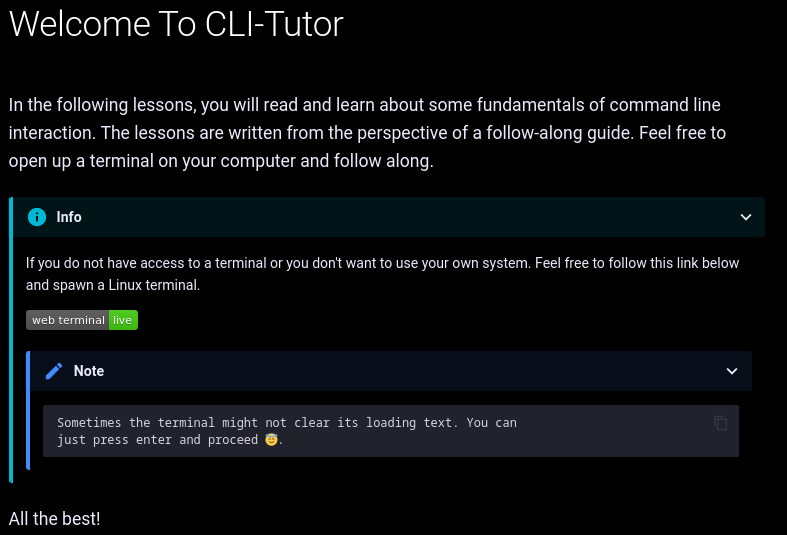
\includegraphics[width=0.85\textwidth]{img/docswelcomedark}
	\caption{Screenshot of the welcome screen of the documentation website, linking to the CLI-only version.}
	\label{fig:cliversion}
\end{figure}

\begin{figure}[htbp]
	\centering
	\includegraphics[width=0.95\textwidth]{img/docs1dark}
	\includegraphics[width=0.95\textwidth]{img/docs1light}
	\caption{Screenshots of the documentation website showcasing both light and dark modes.}
	\label{fig:docsweb}
\end{figure}
